\documentclass[mathserif]{beamer}

\setbeamertemplate{frametitle}[default][center]%Centers the frame title.
\setbeamertemplate{navigation symbols}{}%Removes navigation symbols.
\setbeamertemplate{footline}{\raisebox{5pt}{\makebox[\paperwidth]{\hfill\makebox[10pt]{\scriptsize\insertframenumber}}}}

\usepackage{amsmath,amssymb,amsthm}
\usepackage{graphicx,array,dsfont}
\usepackage{harvard}
\citationmode{abbr}

\newcommand{\Hrule}{\rule{\linewidth}{0.2pt}}
\newcommand{\argmax}{\mathop{\mathrm{argmax}}}
\newcommand{\argmin}{\mathop{\mathrm{argmin}}}
\newcommand{\minimize}{\mathop{\mathrm{minimize}}}
\def\half{\frac{1}{2}}
\def\th{\mathrm{th}}
\def\sign{\mathrm{sign}}
\def\supp{\mathrm{supp}}
\def\E{\mathrm{E}}
\def\P{\mathrm{P}}
\def\Var{\mathrm{Var}}
\def\Cov{\mathrm{Cov}}
\def\R{\mathds{R}} 
\def\cA{\mathcal{A}}
\def\cB{\mathcal{B}}
\def\cE{\mathcal{E}}
\def\cF{\mathcal{F}}
\def\cG{\mathcal{G}}
\def\cN{\mathcal{N}}
\def\red{\color[rgb]{0.8,0,0}}
\def\white{\color[rgb]{1,1,1}}

\begin{document}

%% Lecture was also too short, again about 65-70
%% minutes. Although I didn't really go over the
%% ``Computation, continued'' slide at all. I 
%% think I should slow down, write stuff on the 
%% board. Honestly not sure how much of it they
%% understood (but it was one of the harder topics). 

\title{PageRank}
\author{Rebecca C. Steorts \\ STA 325}
\date{Supplemental Material}

\begin{frame}
\titlepage
{\it Optional reading: ESL 14.10}
\end{frame}

\begin{frame}
\frametitle{Information retrieval with the web}
Last time: {\red information
retrieval}, learned how to compute similarity
scores (distances) of documents to a given 
query string

\bigskip
But what if documents are {\red webpages,} and our 
collection is the whole web (or a big chunk of it)?
Now, two problems:
\begin{itemize}
\item Techniques from last lectures 
(normalization, IDF weighting) are 
{\red computationally infeasible} 
at this scale. There are about 30
billion webpages!
\item Some webpages should be assigned more
{\red priority} than others, for being 
more important
\end{itemize}

\bigskip
Fortunately, there is an underlying structure that 
we can exploit: {\red links between webpages}
\end{frame}

\begin{frame}
\frametitle{Web search before Google}
\begin{center}
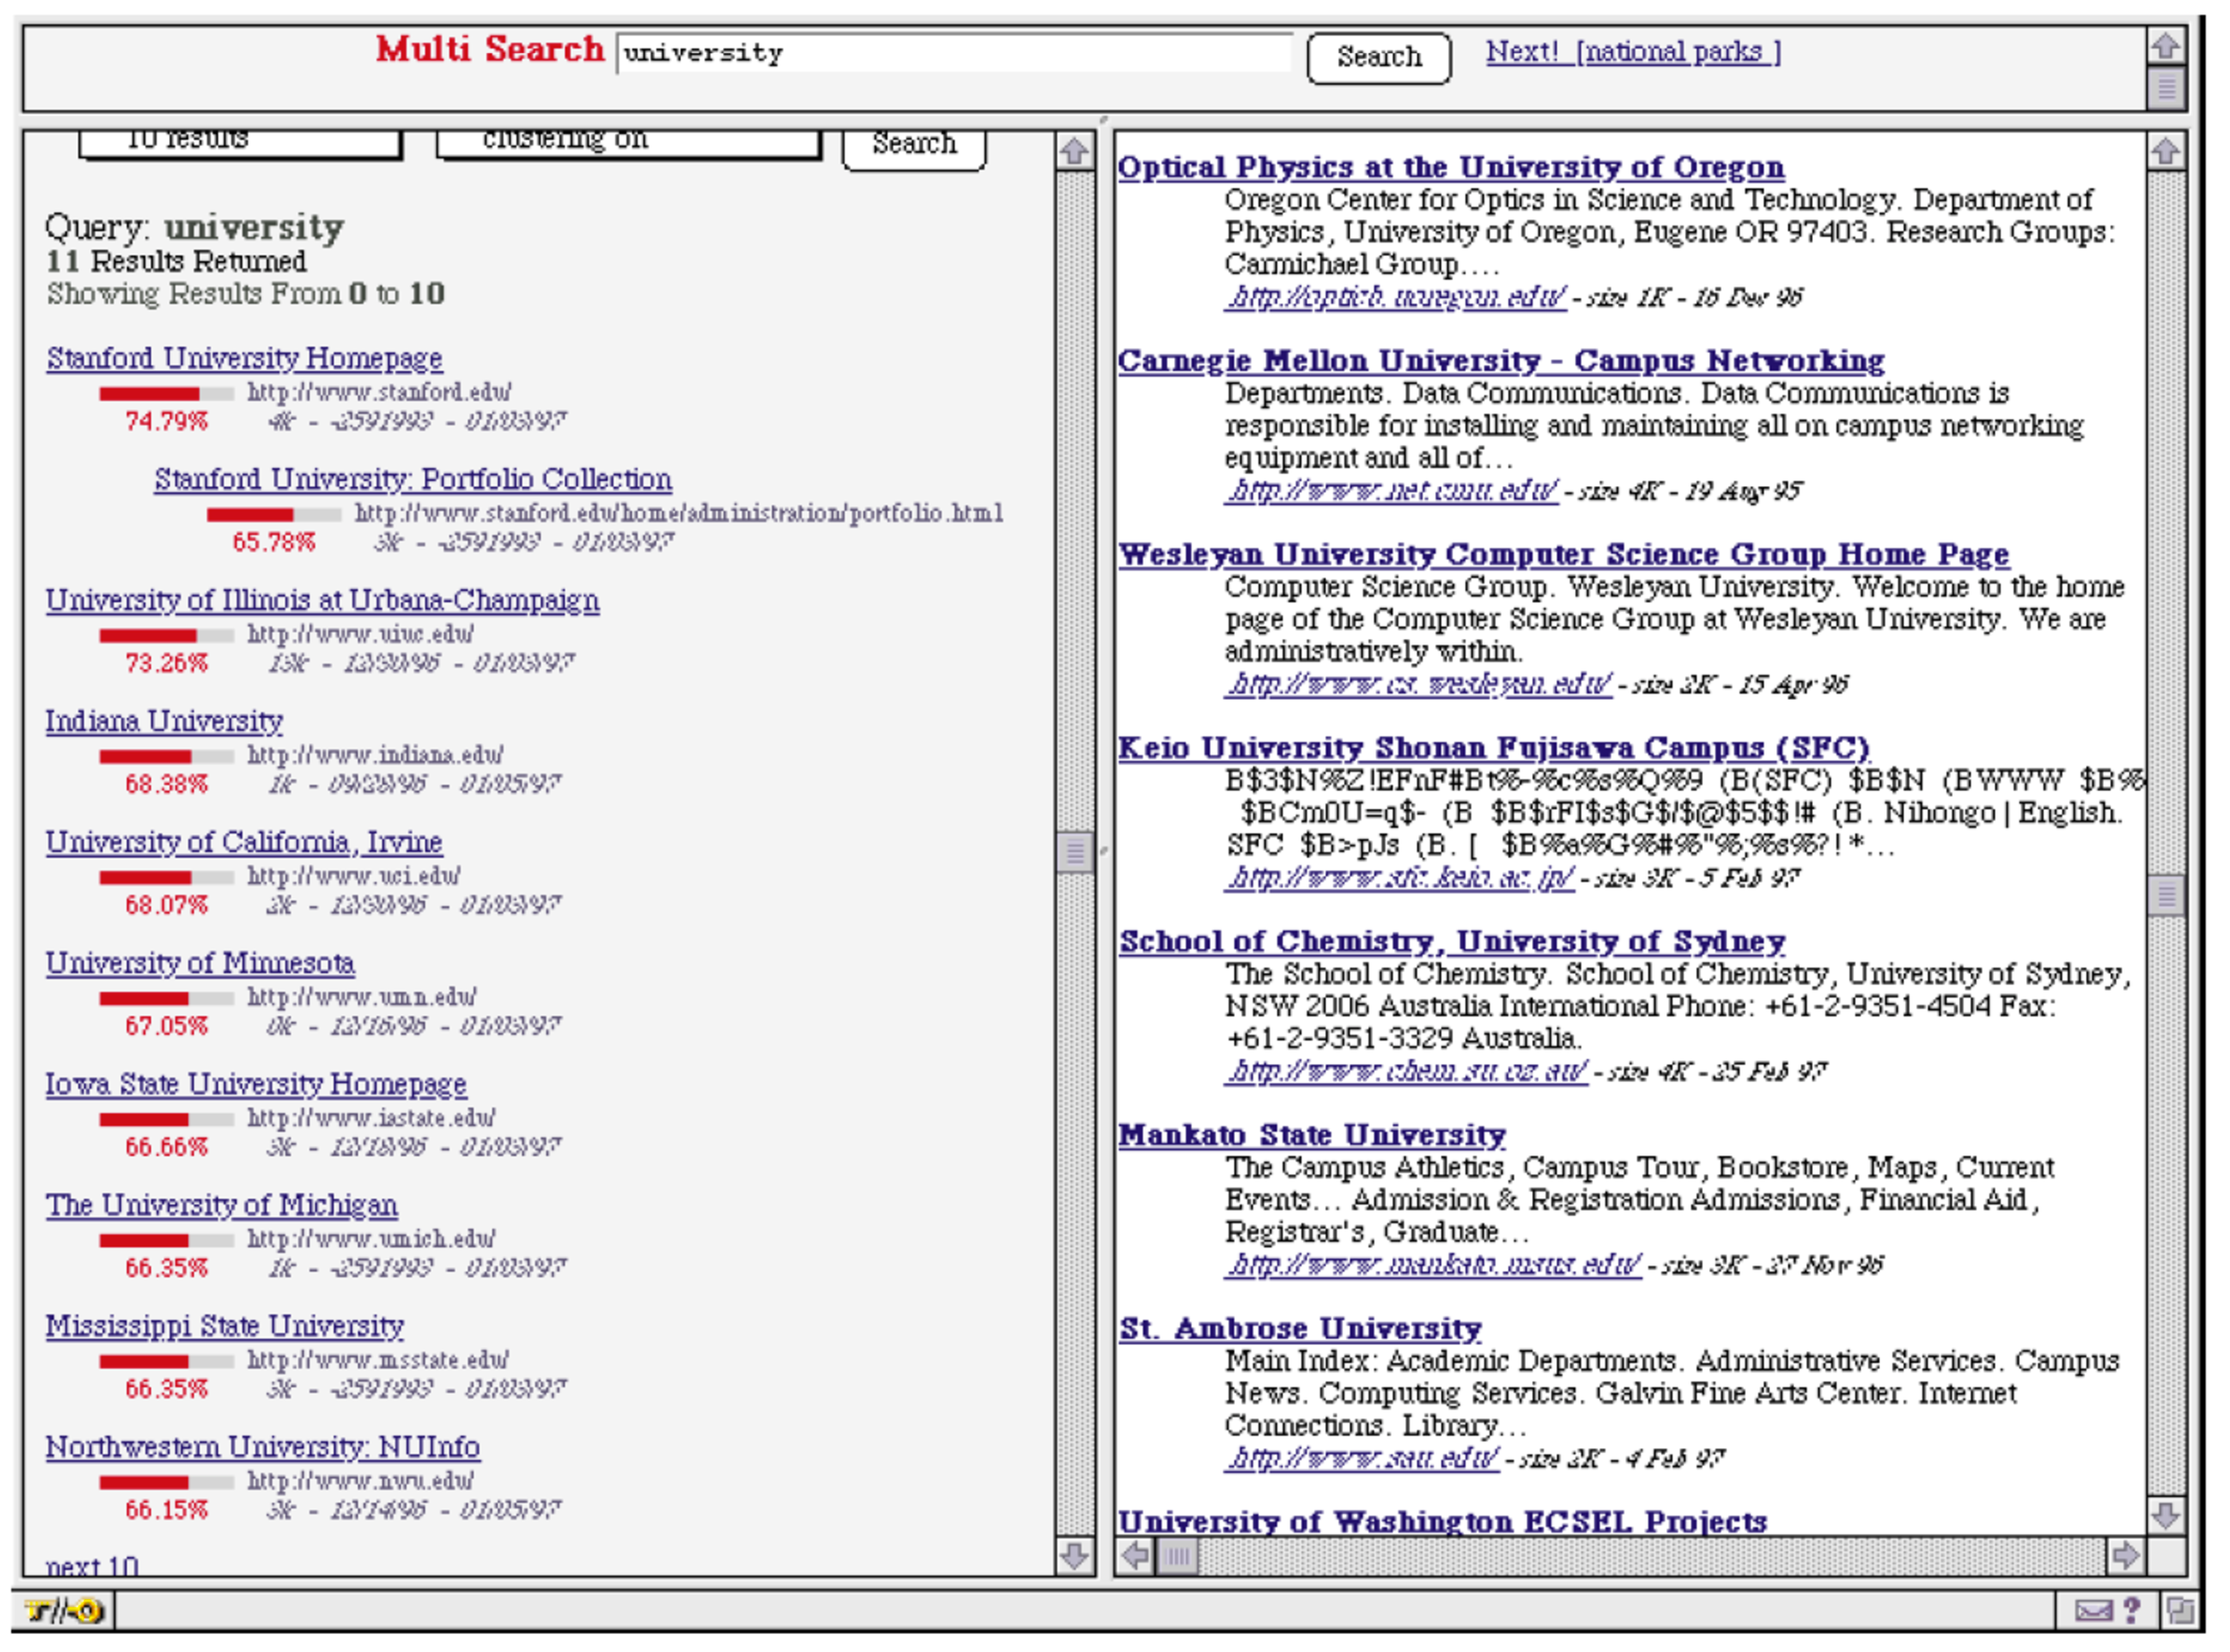
\includegraphics[width=3.5in]{pagerank.pdf}
\end{center}
\vspace{-5pt}
(From Page et al. (1999), ``The PageRank Citation Ranking:
Bringing Order to the Web'')
% http://ilpubs.stanford.edu:8090/422/1/1999-66.pdf
\end{frame}

\begin{frame}
\frametitle{PageRank algorithm}
{\red PageRank algorithm}: famously invented 
by Larry Page and Sergei Brin, founders of Google.
Assigns a {\it PageRank} 
(score, or a measure of importance) to each webpage

\bigskip
\begin{itemize}
\item Suppose there are $n$ webpages.
\item The PageRank of webpage $i$ is based on its 
{\red linking webpages} (webpage(s) $j$ that link to $i$),
\item  Don't just count the number of linking 
webpages, i.e., don't want to treat all linking webpages 
equally
\end{itemize}

\bigskip
Instead, we {\red weight} the links 
from different webpages
\begin{itemize}
\item Webpages that link to $i$, and have high
PageRank scores themselves, should be given
{\red more weight} 
\item Webpages that link to $i$, but link to 
a lot of other webpages in general, should be
given {\red less weight}
\end{itemize}

\bigskip
Note that the first idea is circular! 
(But that's OK)
\end{frame}

\begin{frame}
\frametitle{BrokenRank (almost PageRank) definition}
Let $L_{ij}=1$ if webpage $j$ links to webpage $i$ 
(written $j \rightarrow i$), and $L_{ij}=0$ otherwise

\bigskip
Also let $m_j = \sum_{k=1}^n L_{kj}$,
the total number of webpages that $j$ links to

\bigskip
First we define something that's almost
PageRank, but not quite, because it's broken. 
The {\red BrokenRank $p_i$} of webpage $i$ is
$$p_i 
= \sum_{j \rightarrow i} \frac{p_j}{m_j}
=\sum_{j=1}^n \frac{L_{ij}}{m_j} p_j$$

\bigskip
Does this {\red match our ideas} from the last 
slide? Yes: for $j \rightarrow i$, the weight is 
$p_j/m_j$---this increases with $p_j$, but 
decreases with $m_j$
\end{frame}

\begin{frame}
\frametitle{BrokenRank in matrix notation}
Written in {\red matrix notation,}
\begin{gather*}
p = \left(\begin{array}{c}
p_1 \\ p_2 \\ \vdots \\ p_n
\end{array}\right), \;\;\;
L = \left(\begin{array}{cccc}
L_{11} & L_{12} & \ldots & L_{1n} \\
L_{21} & L_{22} & \ldots & L_{2n} \\
\vdots & & & \\
L_{n1} & L_{n2} & \ldots &  L_{nn}
\end{array}\right), \\
M = \left(\begin{array}{cccc}
m_1 & 0 & \ldots & 0 \\
0 & m_2 & \ldots & 0 \\
\vdots & & & \\
0 & 0 & \ldots & m_n
\end{array}\right)
\end{gather*}
Dimensions: $p$ is $n \times 1$, $L$ and $M$ are 
$n \times n$

\bigskip
Now re-express definition on the previous
page: the {\red BrokenRank vector $p$} is defined as
$p = LM^{-1} p$
\end{frame}

\begin{frame}
\frametitle{Eigenvalues and eigenvectors}
\begin{itemize}
\item Let $A=LM^{-1}$.
\item Then A is a diagonal matrix and $p=Ap$. 
\item This means that $p$ is an 
{\red eigenvector} of the matrix $A$ with {\red eigenvalue 
$1$}.
\end{itemize}

\bigskip
Great! Because we know how to compute the eigenvalues
and eigenvectors of $A$, and there are even methods
for doing this quickly when $A$ is {\red large
and sparse} (why is our $A$ sparse?)

\bigskip
But wait ... do we know that $A$ has an eigenvalue 
of 1, so that such a vector $p$ exists? 
And even if it does exist, will it be unique (well-defined)? 

\bigskip
For these questions, it helps to interpret 
BrokenRank in terms of a {\red Markov chain}
\end{frame}

\begin{frame}{BrokenRank as a Markov chain}
\smallskip

$$A = LM^{-1} \quad \text{and} \quad P = A^{T}$$

\begin{itemize}
\item Big picture: A Markov chain says that the probability of moving from state $i$ to $j$ only depends on state $j.$ 
\item (It doesn't depend anywhere you were before!).
\item Think of a {\red Markov Chain} as a
random process that moves between states
numbered $1,\ldots n$ (each step of the
process is one move).
\item For a Markov chain to have an
$n \times n$
transition matrix $P$, this means 
$$\P(\text{go from $i$ to $j$}) = P_{ij}$$
\end{itemize}

\end{frame}

\begin{frame}{BrokenRank as a Markov chain}
\begin{itemize}
\item Let $p^{(0)}$ is an $n$-dimensional 
vector giving initial probabilities. 
\item After one
step, $p^{(1)} = P^T p^{(0)}$ gives probabilities of being in each
state (why?)
\end{itemize}

As an example:
Let $p^{(0)} = (1/n, \ldots, 1/n).$
Then $p^{(1)} = P_n^T p^{(0)}$
and $p_i^{(1)} = \sum_{j=1}^n P_{ji} p_j^{(0)}.$

\bigskip
\begin{itemize}
\item Now consider a Markov chain, with the states
as webpages, and with {\red transition matrix $A^T$.} 
\item Note that $(A^T)_{ij}=A_{ji}=L_{ji}/m_i$,
so we can describe the chain as
\vspace{-5pt}
$$ P_{ij} = \P(\text{go from $i$ to $j$}) =
\begin{cases}
1/m_i & \text{if $i \rightarrow j$} \\
0 & \text{otherwise}
\end{cases}
\vspace{-5pt}$$
\item (Check: does this make sense?)
This is like a {\red random surfer,}
i.e., a person surfing the web by clicking
on links uniformly at random
\end{itemize}
\end{frame}

%\begin{frame}{BrokenRank as a Markov chain}
%Let $p^{(0)} = (1/n, \ldots, 1/n)$
%Then $p^{(1)} = P_n^T p^{(0)}$
%In general p_i^{(1)} = \sum_{j=1}^n P_{ji} p_j^{(0)}.$
%\end{frame}

\begin{frame}
\frametitle{Stationary distribution}
\smallskip
\smallskip
A {\red stationary distribution} of our Markov 
chain is a probability vector $p$ (i.e., its 
entries are $\geq 0$ and sum to $1$) with
$p = P^Tp$ (Here, we have p = Ap). 

%\bigskip
%I.e., distribution after one step of the Markov chain is
%unchanged. Exactly what we're looking for:
%an eigenvector of $A$ corresponding to eigenvalue $1$

\bigskip
If the Markov chain is {\red strongly connected},
meaning that any state can be reached from any
other state, then stationary distribution $p$ 
exists and is {\red unique}.
% See Theorem 3.1 on page 194 of Bremaud
Furthermore, we can think of the stationary 
distribution as the of proportions of visits the chain 
pays to each state after a very long time 
(the ergodic theorem):

$$p_i = \lim_{t \rightarrow \infty} 
\frac{\text{\# of visits to state $i$ in $t$ steps}}{t}$$
% See Theorem 4.1 on page 111 of Bremaud

\bigskip
{\red Our interpretation}: the BrokenRank of $p_i$ is
the proportion of time our random surfer spends on 
webpage $i$ if we let him go forever
\end{frame}

\begin{frame}
\frametitle{Why is BrokenRank broken?}
There's a {\red problem} here. Our Markov chain---a random
surfer on the web graph---is not strongly 
connected, in three cases (at least):

\bigskip
\begin{tabular}{ccc}
\hspace{-10pt}
\parbox{0.2\textwidth}{\centering
Disconnected components} & Dangling links & Loops 
\smallskip \\
\hspace{-10pt}
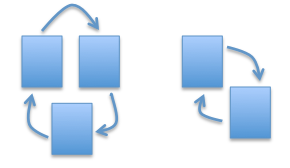
\includegraphics[height=0.9in]{disconnected.png} &
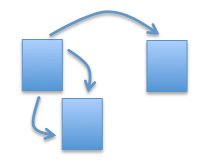
\includegraphics[height=0.9in]{dangling.png} &
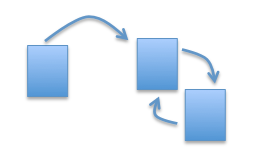
\includegraphics[height=0.9in]{loop.png}
\end{tabular}

\bigskip
Actually, even for Markov chains that are not strongly
connected, a stationary distribution always exists,
% This is by Brouwer fixed-point theorem
but may {\red nonunique} 

\bigskip
In other words, the BrokenRank vector $p$ exists but
is {\red ambiguously defined}
\end{frame}

\begin{frame}
\frametitle{BrokenRank example}
\smallskip
\begin{tabular}{cc}
\hspace{-15pt}
\parbox{0.33\textwidth}{
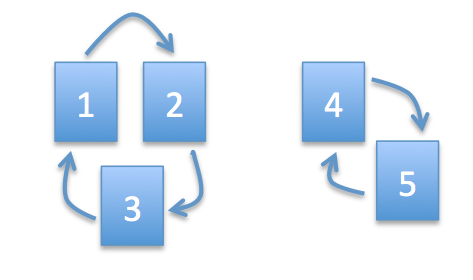
\includegraphics[height=1in]{disconnected-big.png}} &
\hspace{15pt}
\parbox{0.66\textwidth}{
Here $A = LM^{-1} = \left(\begin{array}{ccccc}
0 & 0 & 1 & 0 & 0 \\
1 & 0 & 0 & 0 & 0 \\
0 & 1 & 0 & 0 & 0 \\
0 & 0 & 0 & 0 & 1 \\
0 & 0 & 0 & 1 & 0 \\
\end{array}\right)$
\smallskip\smallskip \\
(Check: matches both definitions?)
}
\end{tabular}

\bigskip
\bigskip
Here there are two eigenvectors of $A$ with 
eigenvalue $1$:
$$p = \left(\begin{array}{c} 
\frac{1}{3} \\ \frac{1}{3} \\ \frac{1}{3} \\ 0 \\ 0
\end{array}\right) \;\;\;\text{and}\;\;\;
p = \left(\begin{array}{c} 
0 \\ 0 \\ 0 \\ \frac{1}{2} \\ \frac{1}{2}
\end{array}\right)$$
These are totally {\red opposite rankings!}
\end{frame}

\begin{frame}
\frametitle{PageRank definition}
{\red PageRank} is given by a small modification of
BrokenRank:
\vspace{-3pt}
$$p_i = \frac{1-d}{n} + d \sum_{j=1}^n
\frac{L_{ij}}{m_j} p_j,
\vspace{-3pt}$$
where $0<d<1$ is a constant 
(apparently Google uses $d=0.85$)

\bigskip
In {\red matrix notation}, this is
\vspace{-3pt}
$$p = \big(\frac{1-d}{n}E + d LM^{-1}\big)p,
\vspace{-3pt}$$
 $E$ is the $n\times n$ matrix of $1$s,
subject to the constraint $\sum_{i=1}^n p_i=1$

\bigskip
(Check: are these definitions the same? Show that 
the second definition gives the first. Hint: if $e$ 
is the $n$-vector of all $1$s, then $E=e e^T$, 
and $e^T p = 1$)
\end{frame}

\begin{frame}
\frametitle{PageRank as a Markov chain}
\begin{itemize}
\item Let $A=\frac{1-d}{n} E + d LM^{-1}$, 
\item Consider a Markov chain with {\red transition
matrix $A^T$} 
\end{itemize}


 $$(A^T)_{ij} = A_{ji} = (1-d)/n + d L_{ji}/m_i$$

$$P_{ij} = \P(\text{go from $i$ to $j$}) =
\begin{cases}
(1-d)/n + d/m_i & \text{if $i \rightarrow j$} \\
(1-d)/n & \text{otherwise}
\end{cases}
$$
\begin{itemize}
\item The chain moves through a link with 
probability $(1-d)/n + d/m_i$, 
\item  with probability 
$(1-d)/n$ it jumps to an unlinked webpage
\item Like a {\red random surfer} with 
{\red random jumps}.
\item Random jumps get rid of our 
problems: our Markov chain is now strongly
connected. 
\item Stationary distribution
(i.e., PageRank vector) $p$ is {\red unique}
\end{itemize}



\end{frame}

\begin{frame}
\frametitle{PageRank example}
\vspace{-5pt}
\parbox{0.3\textwidth}{
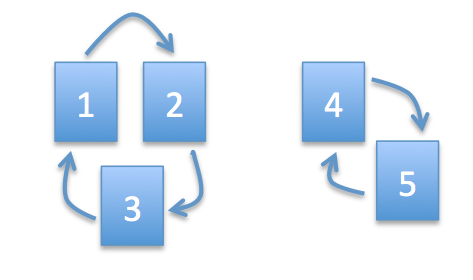
\includegraphics[width=0.3\textwidth]{disconnected-big.png}}
\hspace{5pt}
With $d=0.85$, $A = \frac{1-d}{n}E + dLM^{-1}$
\vspace{-5pt}
\begin{align*}
&=
\frac{0.15}{5} \cdot
\left(\begin{array}{ccccc}
1 & 1 & 1 & 1 & 1 \\
1 & 1 & 1 & 1 & 1 \\
1 & 1 & 1 & 1 & 1 \\
1 & 1 & 1 & 1 & 1 \\
1 & 1 & 1 & 1 & 1 \\
\end{array}\right) + 
0.85 \cdot 
\left(\begin{array}{ccccc}
0 & 0 & 1 & 0 & 0 \\
1 & 0 & 0 & 0 & 0 \\
0 & 1 & 0 & 0 & 0 \\
0 & 0 & 0 & 0 & 1 \\
0 & 0 & 0 & 1 & 0 \\
\end{array}\right) \\
& = 
\left(\begin{array}{ccccc}
0.03 & 0.03 & 0.88 & 0.03 & 0.03 \\
0.88 & 0.03 & 0.03 & 0.03 & 0.03 \\
0.03 & 0.88 & 0.03 & 0.03 & 0.03 \\
0.03 & 0.03 & 0.03 & 0.03 & 0.88 \\
0.03 & 0.03 & 0.03 & 0.88 & 0.03 \\
\end{array}\right)
\end{align*}

\vspace{-25pt}
Now {\red only one} eigenvector of $A$ 
with eigenvalue $1$:
$p=
\left(\begin{array}{c} 0.2 \\ 0.2 \\ 0.2 \\ 0.2 \\ 0.2
\end{array}\right)$
\end{frame}

\begin{frame}
\frametitle{Computing the PageRank vector}
\smallskip
Computing the PageRank vector $p$ via
traditional methods, i.e., an eigendecomposition, 
takes roughly $n^3$ operations.
When $n=10^{10}$, $n^3=10^{30}$.
Yikes! (But a bigger concern would be memory ...)

\bigskip
Fortunately, {\red much faster} way
to compute the eigenvector of $A$ with eigenvalue $1$:
begin with {\red any initial distribution $p^{(0)}$},
and compute
\begin{align*}
p^{(1)} &= A p^{(0)} \\
p^{(2)} &= A p^{(1)} \\
&\vdots  \\
p^{(t)} &= A p^{(t-1)}, 
\vspace{-10pt}\end{align*}
Then $p^{(t)} \rightarrow p$ as $t \rightarrow \infty$. 
% By Perron-Frobenius
In practice, we just repeatedly multiply by $A$ until
there isn't much change between iterations

\bigskip
E.g., after 100 iterations, operation count: $100n^2 
\ll n^3$ for large $n$
\end{frame}

\begin{frame}
\frametitle{Computation, continued}

There are still important questions remaining about 
computing the PageRank vector $p$ (with the algorithm
presented on last slide):
\begin{enumerate}
\item How can we perform each iteration quickly 
(multiply by $A$ quickly)?
\item How many iterations does it take (generally)
to get a reasonable answer?
\end{enumerate}

\bigskip
Broadly, the answers are:
\begin{enumerate}
\item Use the {\red sparsity of web graph} (how?)
\item Not very many if $A$ large {\red spectral gap}
(difference between its first and second largest
absolute eigenvalues); the largest is $1$, the second 
largest is $\leq d$
%http://www-cs-students.stanford.edu/~taherh/papers/secondeigenvalue.pdf
\end{enumerate}

\bigskip
(PageRank in R: see the function {\tt page.rank} in 
package {\tt igraph})
\end{frame}

\begin{frame}
\frametitle{A basic web search}
\smallskip
For a basic web search, given a query, we could do the 
following:
\begin{enumerate}
\item Compute the PageRank vector $p$ {\red once} 
(Google recomputes this from time to time, to stay current)
\item Find the documents containing all words in the query
\item {\red Sort} these documents {\red by PageRank}, and
return the top $k$ (e.g., $k=50$) 
\end{enumerate}

\bigskip
This is a little too simple ... but we can use
the {\red similarity scores} learned last time,
changing the above to:
\begin{itemize}
\item[3.] Sort these documents by PageRank, and keep only the 
top $K$ (e.g., $K=5000$)
\item[4.] {\red Sort by similarity} to the query 
(e.g., normalized, IDF weighted distance), 
and return the top $k$ (e.g., $k=50$)
\end{itemize}

\bigskip
Google uses a combination of PageRank, similarity scores,
and other techniques (it's proprietary!)
\end{frame}

\begin{frame}
\frametitle{Variants/extensions of PageRank}
\smallskip
A precursor to PageRank:
\begin{itemize}
\item {\red Hubs and authorities}: using link structure to determine
``hubs'' and ``authorities''; a similar algorithm was used
by Ask.com
{\scriptsize(Kleinberg (1997), ``Authoritative Sources in a Hyperlinked Environment'')}
\end{itemize}

\smallskip
\smallskip
Following its discovery, there has been a huge amount of work 
to improve/extend PageRank---and not only at Google! There are many,
many academic papers too, here are a few:
\begin{itemize}
\item {\red Intelligent surfing}: pointing surfer towards textually
relevant webpages
{\scriptsize (Richardson and Domingos (2002), ``The Intelligent Surfer: 
Probabilistic Combination of Link and Content Information in PageRank'')}
\item {\red TrustRank}: pointing surfer away from spam
{\scriptsize (Gyongyi et al. (2004), ``Combating Web Spam with TrustRank'')}
\item {\red PigeonRank}: pigeons, the real reason for Google's success
{\scriptsize(\url{http://www.google.com/onceuponatime/technology/pigeonrank.html})}
% http://www.math.cornell.edu/~mec/Winter2009/RalucaRemus/
\end{itemize}
\end{frame}

% \begin{frame}
% \frametitle{Encouragement}
% \smallskip
% (I {\it don't} mean:
%  ``Google found the $25$ billion dollar eigenvector.'')
% \begin{center}
% 
\includegraphics[width=2in]{study.jpg}
% \end{center}
% ``Beautiful math tends to be useful, and useful things tend
% to have beautiful math.'' ...
% Statistics is often where it comes together.
% \end{frame}

\begin{frame}
\frametitle{Recap: PageRank}
{\red PageRank} is a ranking algorithm for webpages based on their 
importance. For a given webpage, its PageRank is based on 
the webpages that link to it; it helps if these 
linking webpages have high PageRank themselves; it hurts
if these linking webpages also link to a lot of other 
webpages

\bigskip
We defined it by modifying a simpler ranking system
({\red BrokenRank}) that didn't quite work.
The PageRank vector $p$ corresponds to the
{\red eigenvector} of a particular matrix $A$ corresponding to
{\red eigenvalue $1$}. Can also be explained in terms of 
a Markov chain, interpreted as a {\red random surfer} with {\red 
random jumps}. These jumps were crucial, because they made the 
chain strongly connected, and guaranteed that the PageRank 
vector (stationary distribution) $p$ is unique

\bigskip
We can compute $p$ by repeatedly multiplying 
by $A$. PageRank can be combined with similarity scores for 
a basic web search
\end{frame}

%\begin{frame}
%\frametitle{Next time: clustering}
%
%\begin{center}
%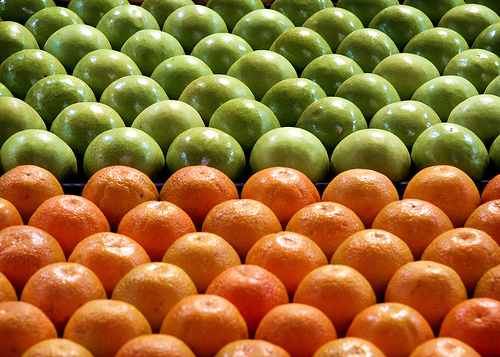
\includegraphics[width=2.5in]{applesoranges.jpg}
%\end{center}
%
%\bigskip
%Not quite as easy as apples with apples and oranges with oranges 
%\end{frame}
\end{document}

